\section{Problem Formulation}
%----------------------------------------------------------------------------------------%
In this section, we formulate the standard MDP problem with respect to global system states and jobs dispatching policy of which is compounded of all AP nodes in this MEC system.
Given the fact that AP nodes would obtain global states update only after \emph{Update Latency} in each broadcast interval, the formulated MDP problem is composed of two adjacent broadcast interval with obsolete information and updated information.
As we allow policy update over partial obsolete information, the formulated MDP problem is further split into two sub-problem leveraging same problem structure. The structure would lead to performance improvement guarantee with the proposed distributed algorithm.
Then we show that the solution for all AP nodes suffers from curse of dimensionality and a low-complexity solution is needed.

\subsection{System State and Dispatching Policy}
The system states is selected based on the nature that $k$-th AP comes up with complete broadcast information only after its corresponding \emph{Update Latency} in the broadcast interval.
The relative difference between broadcast point and the update time point is depicted in Fig. \ref{fig:brd-trans}.
\begin{definition}[System State]
    The system state at $i$-th broadcast point is denoted as $\Stat_i \define (\Obsv_{i-2}, \Obsv_{i-1}, \Obsv_{i}), (i=1,2,\dots)$, where $\Obsv_{-1}=\Obsv_{0} =\Phi$ denotes the empty system state.
    $\Obsv_{i}$ denotes updated information after receiving global broadcasting information, $\Obsv_{i-1}$ denotes the partial stale information, and $\Obsv_{i-2}$ denotes the more stale information which have impact on transition function with respect to $\Obsv_{i-2}$.
\end{definition}

\begin{figure}[ht]
    \centering
    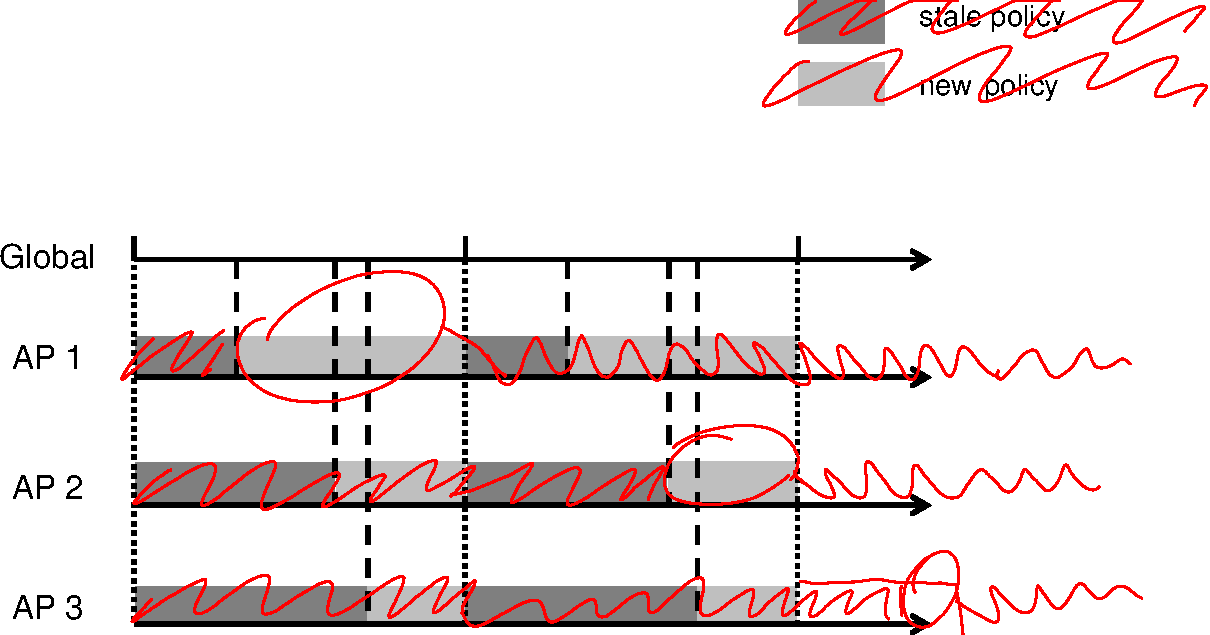
\includegraphics[width=0.45\textwidth]{brd-trans.pdf}
    \caption{Global System Transition with Partial Information-based Dispatching Decision}
    \label{fig:brd-trans}
\end{figure}

The \emph{dispatching policy} is applied over arrival jobs in each timeslot on each AP, and thus \emph{dispatching action space} is defined as $\mathbf{A}: (j, m) \in \jSpace \times \esSet$ where $(j, m)$ denotes the action that $j$-type job should be uploaded to $m$-th ES.
\begin{definition}[Update Time Points]
    For $k$-th AP ($\forall k\in\apSet$), partial updates firstly and then consensus update, which is defined as follows.
    \begin{itemize}
        \item Partial Update Point: The AP nodes will update their own policy when the corresponding \emph{Maximum Broadcast Latency} is achieved, and awareness of the previous policy change for the AP nodes receiving information before it;
        \item Iterative Update Points: When reaching the ending of the broadcast interval, all the AP nodes would update the policy together;
        this policy iteration is evaluated with no policy changes consideration in the following time in this interval;
        this policy iteration is with partial information only with last interval, but not with information from this interval.
    \end{itemize}
\end{definition}
        
Based on the three stages of global system information defined in system state, the compounded global-wise policy of all AP nodes is defined as follows.
\begin{definition}[Compounded Dispatching Policy]
    The compounded dispatching policy $\Policy(\Stat_{i})$ over $\Stat_{i}$ which is defined with three-stage broadcasting information which is given as follows.
    \begin{align}
        \Policy(\Stat_{i}) \define \Bracket{
            \Omega'(\Obsv_{i-2}), \Omega(\Obsv_{i-1}), \Omega'(\Obsv_{i-1}), \Omega(\Obsv_{i}),
        }
    \end{align}
    where $\Omega'(\Obsv_i) \define [\tilde{\Omega}'_{1}(\Obsv_i), \dots, \tilde{\Omega}'_{K}(\Obsv_i)]$ denotes the policy applied at \emph{Partial Update Point} with obsolete partial information; and $\Omega(\Obsv_i) \define [\tilde{\Omega}_{1}(\Obsv_i), \dots, \tilde{\Omega}_{K}(\Obsv_i)]$ denotes the policy at \emph{Iterative Update Points} respectively, i.e. $k$-th AP ($\forall k\in\apSet$) would change its policy from $\tilde{\Omega}_{k}'(\Obsv_i)$ to $\tilde{\Omega}_{k}(\Obsv_{i+1})$ when receiving information $\Obsv_{i+1}$ while the others keep their own policy.
            
    Furthermore, the local policy for AP nodes is defined according to \emph{dispatching action space} as follows.
    \begin{align}
        &\tilde{\Omega}_{k}(\Obsv_{i}) \define \set{\omega^{(i)}_{k,j}(m)|\forall j\in\jSpace, \forall m\in\esSet}
        ~(\forall k\in\apSet)
        \\
        &\tilde{\Omega}'_{k}(\Obsv_{i}) \define \set{\omega'^{(i)}_{k,j}(m)|\forall j\in\jSpace, \forall m\in\esSet}
        ~(\forall k\in\apSet),
    \end{align}
    where $\omega^{(i)}_{k,j}(m)$ denotes the deterministic dispatching policy that: when $k$-th AP with information $\Obsv_{i}$ after its iterative update point, it would then upload $j$-type job to $m$-th ES if and only if $\omega^{(i)}_{k,j}(m)=1$; $\tilde{\Omega}'_{k}(\Obsv_i)$ is for partial update point.
\end{definition}

More specifically, the multiple-phase of the policy $\tilde{\Omega}_k(\Obsv_i)$ at multiple \emph{iterative update points} are separated by \emph{Update Latency} $d_{k}$ for $k$-th AP ($k\in\apSet$). One vivid example of policy adaption phase is given as follows, the update rules of which will be elaborated in next sub-section.
\begin{example}[Policy Phase Adaption]
    In the time interval $[t_{i}, t_{i+1}]$, $k$-th AP would adopt $\tilde{\Omega}_{k}'(\Obsv_{i-1})$ immediately after $t_i$, and adopt $\tilde{\Omega}_{k}(\Obsv_{i})$ after its corresponding iterative update points; then with $\tilde{\Omega}_{k}'(\Obsv_{i})$ at $t_{i+1}$ and repeat the process.
\end{example}
%----------------------------------------------------------------------------------------%

\subsection{The Optimization Problem}
We propose the jobs dispatching optimization problem with the target to minimize \emph{average response time} of all offloaded jobs in MEC system.
The \emph{average response time} is composed of uploading time from $AP$ to $ES$, and queueing-and-service time on corresponding ES. According to \emph{Little's Law}, the average response time of all jobs is equally as average number of jobs in system.
        
Due to the intrinsic property of periodic information broadcasting, we collect the cost for number counting at the pace of broadcasting interval which could be seems as sampling of original process based on timeslot scale.
Besides the cost counted for job response time, we furthermore add penalty on jobs submission over its capacity limit when the over-limited jobs will be rejected at the end of current broadcast interval.
Therefore, the cost function of this problem is given as follows.
\begin{align}
    g\Paren{\Stat_{i}, \Policy(\Stat_{i})} \define& \sum_{k\in\apSet}\sum_{m\in\esSet} \Inorm{\vec{r}^{(k)}_{m}(i)} + \sum_{m\in\esSet}\sum_{j\in\jSpace}
    \nonumber\\
    &\Brace{
        q_{m,j}(i) + \beta I[q_{m,j}(i)=L_Q]
    },
\end{align}
where $\Inorm{\vec{r}^{(k)}_{m}}$ denotes the $L^1$-norm of vector $\vec{r}^{(k)}_{m}$, i.e. the sum up of absolute value of each entry; $\beta$ are weight factor for full-queue penalty.
        
Our distributed optimization problem definition is given as follows.
\begin{problem}[Original Cooperative Job Dispatching Problem]
    \begin{gather}
        \min_{\Policy} \lim_{T \to \infty}
            \mathbb{E}_{\Policy}
                \Bracket{\sum_{i=2}^{T} \gamma^{i-1} g(\Stat_{i}, \Policy(\Stat_{i}))|\Stat_1},
    \end{gather}
    where the cost is collected with a discount factor $\gamma$, and $\Policy$ is optimized globally always with full-state information available.
\end{problem}
According to \cite{sutton1998introduction}, the above problem could be solved by the following \emph{Bellman's equation}:
\begin{align}
    V(\Stat_i) =& g(\Stat_i) +
        \nonumber\\
        &\gamma \min_{\Policy(\Stat_{i})} \sum_{\Stat_{i+1}} \Pr\{ \Stat_{i+1}|\Stat_{i}, \Policy(\Stat_{i}) \} V(\Stat_{i+1}).
    \label{sp0}
\end{align}
        
However, the state information is actually partial-presence as $(\Obsv_{i-1}, \Obsv_{i-2})$ at $t_i$ while $\Obsv_{i}$ would be available only after the corresponding \emph{Maximum Broadcast Latency} for each AP nodes.
This problem structure results into different information knowledge on \emph{Partial Update Point} and \emph{Iterative Update Points} in this interval.
Thus we decouple the original problem into two sub-MDP problem in a successively update style.
        
The first problem solves policy update at \emph{Partial Update Point} which assumes no policy update at \emph{Iterative Update Points}. The corresponding Bellman's Equation is defined as follows.
\begin{align}
    V(\Stat_i) = g(\Stat_i) + \gamma \min_{\Omega'(\Obsv_{i-1})} \Pr\{ \Obsv_{i+1}|\Obsv_{i-1}, \Policy(\Stat_i) \} V(\Stat_{i+1}),
    \label{sp1}
\end{align}
where $\Policy(\Stat_i) = [\Omega'(\Obsv_{i-2}), \Omega(\Obsv_{i-1}), \Omega'(\Obsv_{i-1}), \Omega'(\Obsv_{i-1})]$ without policy update in $(t_i, t_{i+1}]$.
        
The second problem solves policy update at \emph{Iterative Update Points} which assumes no policy update at \emph{Partial Update Points}.
Furthermore, the update is applied iteratively, as the name implies, with the order following length of broadcast latency (i.e. the sorted AP nodes order). The corresponding Bellman's Equation for $k$-th AP ($\forall k\in\apSet$) node is defined as follows.
\begin{align}
    V(\Stat_i) = g(\Stat_i) + \gamma \min_{\Omega^{(k)}(\Obsv_{i})} \Pr\{ \Obsv_{i+1}|\Obsv_{i}, \Policy(\Stat_i) \} V(\Stat_{i+1}),
    \label{sp2}
\end{align}
where $\Omega^{(k)}(\Obsv_{i}) = [\tilde{\Omega}_{1}(\Obsv_{i}), \dots, \tilde{\Omega}_{k}(\Obsv_{i}), \tilde{\Omega}_{k+1}(\Obsv'_{i-1}), \dots, $ $\tilde{\Omega}_{K}(\Obsv'_{i-1})]$ in $\Policy(\Stat_i)$.
It implies that the updated policy before $k$-th AP must be known and thus impact the transition function of $k$-th AP.
        
The two sub-problem are applied successively, with policy improvement based on last policy update. The performance improvement of next policy update is guaranteed by optimal solution of Bellman's Equation with fixed policies from previous update.
To better analyze the optimization structure of the two sub-problem, we decouple the 
We note that after the dispatching policy, the arrival distribution $A_{k,j}$ is further split onto different Edge Servers. The split arrival processes for $k$-th AP ($\forall k\in\apSet$) are still i.i.d Poisson Point Processes but with different arrival rates as $\set{\lambda_{k,j}I[\omega^{(i)}_{k,j}(m)=1]|\forall m\in\esSet}$ ($I[\cdot]$ is indicator function). The decoupled expression of transition function of Eqn. \ref{sp1} and Eqn. \ref{sp2} is given as follows.
        
\begin{lemma}[Transition Function Decoupling]
    The transition function in Bellman's equation could be decoupled on AP nodes states and ES nodes states, which will facilitate the approximated value function expression in the following section.
    The decoupled transition function for Eqn. \ref{sp1} is given as follows.
    \begin{align}
        & \Pr\{\Obsv_{i+1}|\Obsv_{i-1}, \Policy(\Stat_{i})\}
        \nonumber\\
        =& \prod_{k\in\apSet}\prod_{m\in\esSet}\prod_{j\in\jSpace}
                \Pr\Brace{r^{(k)}_{m,j}(i+1)|\tilde{\Omega}'_k(\Obsv_{i-1})}
                \times \prod_{m\in\esSet}\prod_{j\in\jSpace}
            \nonumber\\
            & \Pr\Brace{Q_{m,j}(i+1)|Q_{m,j}(i-1), \set{r^{(k)}_{m,j}(i-1)|\forall k\in\apSet},
            \nonumber\\
            & \Omega'(\Obsv_{i-2}), \Omega(\Obsv_{i-1}), \Omega'(\Obsv_{i-1})}.
    \end{align}
    And the decoupled transition function for Eqn. \ref{sp2} is given as follows.
    \begin{align}
        & \Pr\{\Obsv_{i+1}|\Obsv_{i}, \Policy(\Stat_{i})\}
        \nonumber\\
        =& \prod_{k\in\apSet}\prod_{m\in\esSet}\prod_{j\in\jSpace}
                \Pr\Brace{ r^{(k)}_{m,j}(i+1) | \Omega^{(k)}(\Obsv_i) }
                \times \prod_{m\in\esSet}\prod_{j\in\jSpace}
            \nonumber\\
            & \Pr\Brace{Q_{m,j}(i+1)|Q_{m,j}(i), \set{r^{(k)}_{m,j}(i)|\forall k\in\apSet},
            \nonumber\\
            & \Omega'(\Obsv_{i-1}), \Omega^{(k)}(\Obsv_{i})}.
    \end{align}
\end{lemma}
\begin{proof}
    \hl{Proof deleted.}
\end{proof}

However, after the state decomposition, the action space would still be exponentially expanded with respect to number AP and ES nodes. We could not use traditional \emph{policy iteration} or \emph{value iteration} algorithm \cite{sutton1998introduction} for unacceptable computational complexity.
So in next section, to alleviate curse of dimensionality, we introduce baseline dispatching policy to approximate the value function, and then carry out one-step iteration to obtain a better value function approximation.
%----------------------------------------------------------------------------------------%